\section{Method} \label{sec:method}
%Method
%Prerequisites (things used by all networks)
%Data set (fruit), (landscape)
%Input size (128X128)
%
%Color spaces + which one to use :
%RGB (luminosity not separated from color)
%HSV (circular domain)
%YCbCr (OK)
%CIELab (OK)
%first layer as input, second and third layer as output
%
%Architecture (not what it is but why WE use it)
%General discription (how to colorize an image with an NN)
%Features used by all networks
%ReLu, weight initialization, padding, kernel size
%Feature extraction
%Reconstruct
%Concatenate
%Dilated convolution
%Color generation
%Two feature maps
%blur
%Classification
%k-means
%annealed mean
%gaussian blur
%
%Loss function
%Squared error
%Class rebalancing (histogram dataset)
%Cross entropy
%Class rebalancing
%Architectures used:
%Dahl, Compact, Dahl_classifier, Dahl_zhang, Zhang
%
%Training method
%nesterov momentum
%adadelta

This section covers the different methods used to get an answer to the question of which CNN setup is best in colorization of images. Firstly, the chosen dataset will be explained. In addition the input size and the different colorspaces used will be explained. Next the different architectures used will be explained. Features extraction, training parameters, loss functions, and general architectures of the chosen networks will be evaluated. Finally the test setup will be explained.

\subsection{Dataset and Input}

Large training and validation datasets are required for training and validation of the CNNs.
Some restrictions on the datasets had to be made due to limitations in computational power, resulting in a selection of images based on a certain category; fruit and landscape images.

The landscape dataset is used as a low-level test case, images of landscapes offer less distinct features coupled to a mapping of the colors, e.g. most landscapes are green at the bottom and blue at the top. The high-level test case consists of the fruit dataset.
Fruit is a category which has distinct colors corresponding to distinct features. Therefore, in order to color fruit correctly, the network has to learn to link colors to distinct features in the input, straining the networks requirements. Also many fruit classes are linked to ambiguous colors, i.e. green or red apple. Taking fruit as the dataset is therefore an excellent method to check whether the network is able to counter the 'averaging' problem also mentioned before.

The datasets are generated using the popular image website Flickr\footnote{\url{https://www.flickr.com/}}.
Using their freely available API, a program was made that retrieved images in the required resolution and kept track of images retrieved, to avoid duplicates. The datasets retrieved had to be checked on incorrect images. To solve this problem a web application was made that enabled us to check images on defects. The checked datasets are collected in batches and stored in Python Numpy arrays as input for the network.
This resulted in 2 datasets, which are summarized in table \ref{tab:dataset}.

\begin{table}[h!]
	\centering
	\caption{Datasets used for training and validation of the various networks}
	\label{tab:dataset}
	\begin{tabular}{|l|l|l|}
		\hline
		\textbf{Dataset}   & \textbf{\# Training Images} & \textbf{\# Validation images} \\ \hline \hline
		Fruit     & 6000            & 1000              \\ \hline
		Landscape & 34000           & 5000              \\ \hline
	\end{tabular}
\end{table}

The network input are 128x128 pixel grayscale images, which are propagated through the network in batches. Using batches reduces computation time since better use is made of the parallelization of modern computer architectures. Most importantly the gradients calculated using batches are a better estimate of the gradient for the entire training set, thus leading to a more stable gradient descent \cite{ioffe2015batch}. Making the batch size too large makes the search to the global minimum less stochastic, thus making it converge to a local optimum more quickly, and in general converging less quickly. 

The network is trained to be able to colorize an image, but the way it outputs the colorized image is dependent on the color space used during training. There are several options available:\\

\textbf{RGB} This widely used color space specifies an intensity for the channels red, blue and green. The biggest drawback of using RGB is that the color is not separated from the luminosity. In this way, the network needs not only to output a hue and saturation of a color, but also the luminosity itself. This makes it a much tougher challenge to output an image that resembles a colorized version of the grayscale image. A visualization of the RGB space is given in figure \ref{fig:RGB}.

\textbf{HSV} Specifying the hue, saturation and value, uncouples the luminosity (value) from the color (hue and saturation). Furthermore decoupling the saturation could allow specifically tackling the sepia and saturation problem as described in section \ref{sec:intro}. However, the color space is periodic in the hue axis. From the numerical perspective, this leads to an ambiguous error specification, since for one difference between target and network output color, two directions of improvement are equally valid, thus a very complicated loss function is required, where the network needs to learn this circular property of the hue axis. This colorspace is used for training on the compact network architecture, however the network did not perform as good as when it was trained on either YCbCr or CIELab. Therefore the HSV colorspace was omitted.

\textbf{YCbCr} The Y channel contains the luminosity of the image, while Cb and Cr layers are the chroma blue and chroma red layers respectively. While providing a separate luminosity channel, it was found that for different Y values, a given Cb and Cr combination does not specify the same color. This makes the error in the color specification dependent on the luminosity of the image. A visualization of the color space can be found in \ref{fig:YCbCr}.

\textbf{CIELab} Similarly to the YCbCr color space, the L channel specifies the luminosity, the a and b layers the color. In contrast with the YCbCr space, a given a and b value specify a color, while the luminosity only determines how light the color is. However, for a single L layer not all a and b value translate to colors that can be represented in the RGB color space (as displayed by computer monitors). The CIELab color space is visualized in figure \ref{fig:CIELab}.\\

To summarize, the HSV, YCbCr and CIELab color spaces all have the possibility of using one channel as input to the neural network, while requiring only two outputs of the network that instead of three with the RGB color space. Combined with the input, these two outputs allow reconstructing a color image. According to Iizuka, the CIELab color space has been found to give the most correct results for a colorization network\cite{IizukaSIGGRAPH2016}. Considering the disadvantages of the HSV color space, the YCbCr and CIELab color spaces are compared during the present research.

\begin{figure}
	\centering
	\begin{subfigure}[b]{0.32\textwidth}
		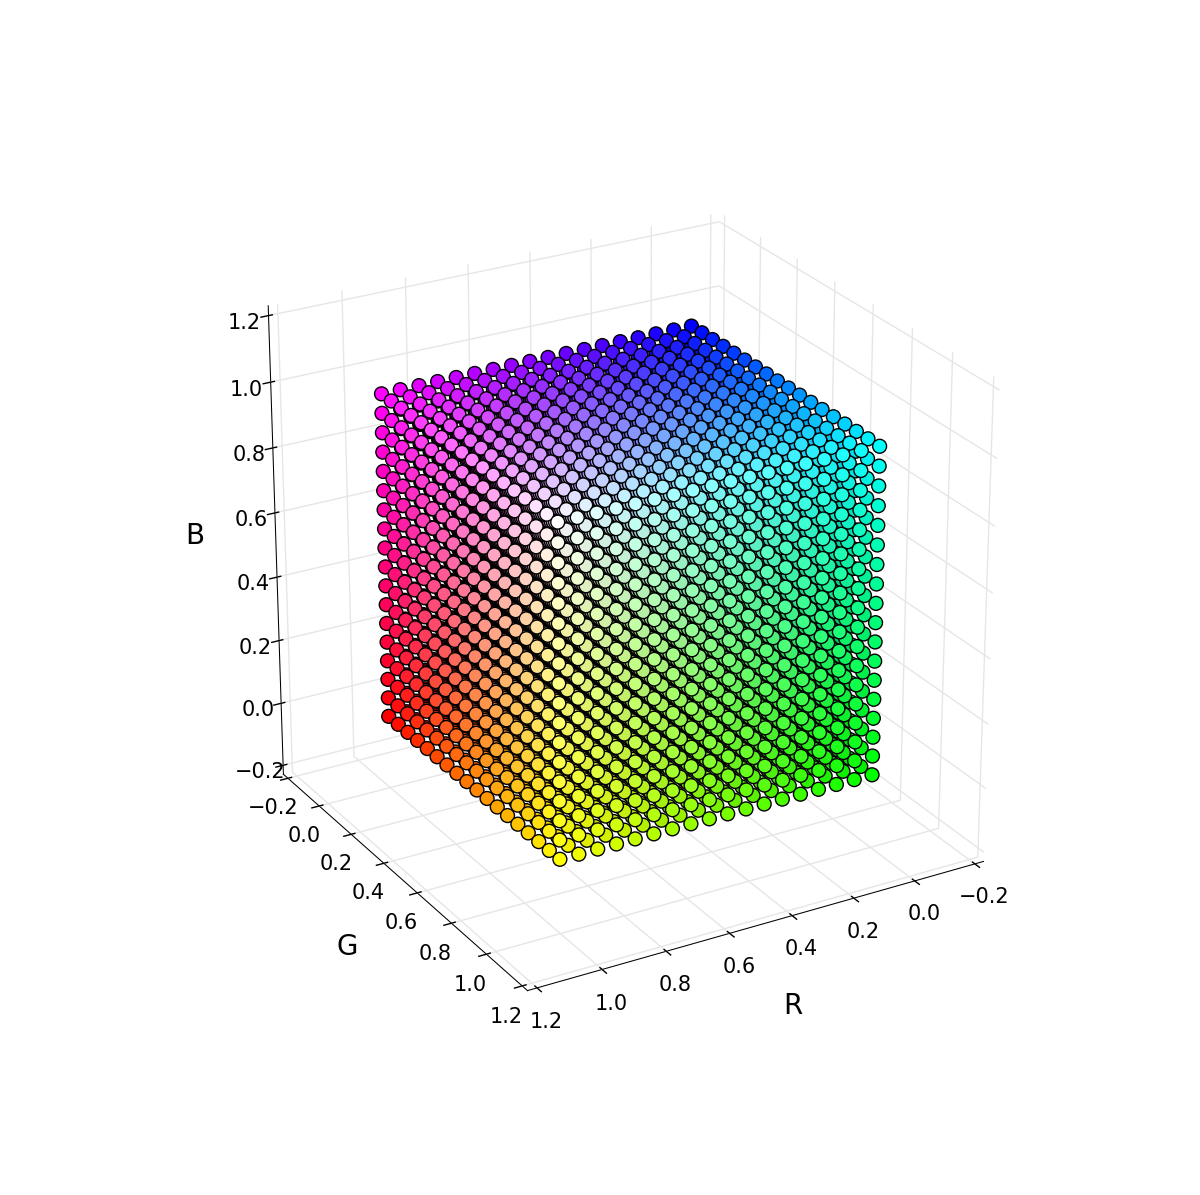
\includegraphics[width=\textwidth,trim={125px 75px 125px 75px},clip]{RGB}
		\caption{The RGB colorspace}
		\label{fig:RGB}
	\end{subfigure}
	~ %add desired spacing between images, e. g. ~, \quad, \qquad, \hfill etc. 
	%(or a blank line to force the subfigure onto a new line)
	\begin{subfigure}[b]{0.32\textwidth}
		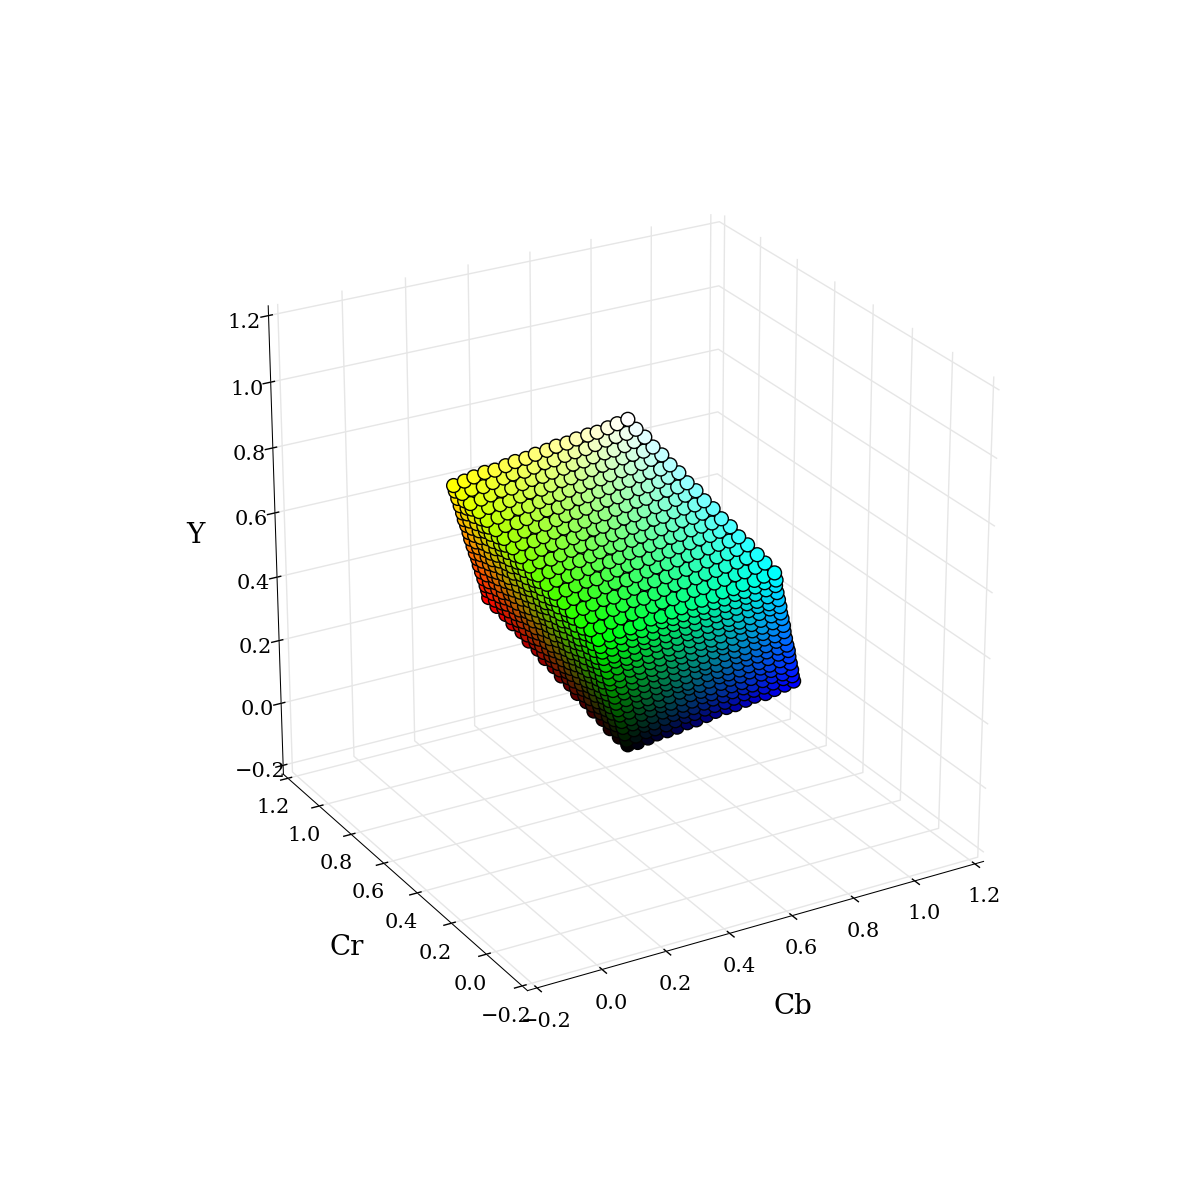
\includegraphics[width=\textwidth,trim={125px 75px 125px 75px},clip]{YCbCr}
		\caption{The RGB colorspace represented in the YCbCr colorspace}
		\label{fig:YCbCr}
	\end{subfigure}
	~ %add desired spacing between images, e. g. ~, \quad, \qquad, \hfill etc. 
	%(or a blank line to force the subfigure onto a new line)
	\begin{subfigure}[b]{0.32\textwidth}
		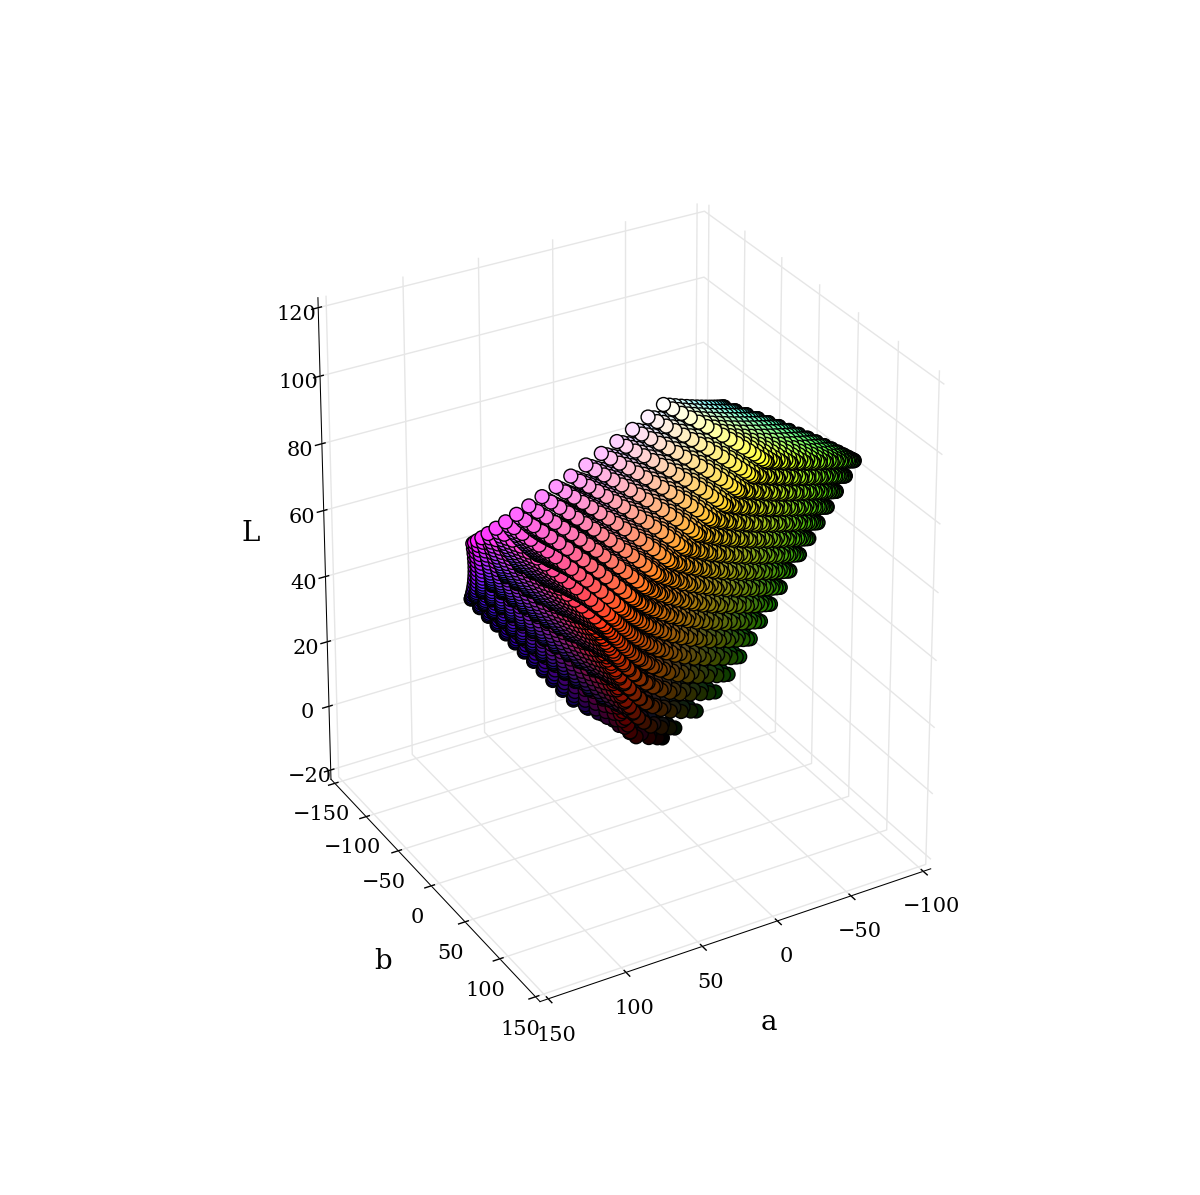
\includegraphics[width=\textwidth,trim={175px 75px 150px 75px},clip]{CIELab}
		\caption{The RGB colorspace represented in the CIELab colorspace}
		\label{fig:CIELab}
	\end{subfigure}
	\caption{The different colorspaces used in the different networks}\label{fig:animals}
\end{figure}

\subsection{Convolutional neural network properties}
\label{sec:nnproperties}

\begin{wrapfigure}{R}{0.5\textwidth}
	\vspace{-20pt}
	\begin{center}
		\includegraphics[width=0.49\textwidth,trim={75px 0px 75px 0px},clip]{K_nearest}
	\end{center}
	\caption{K nearest neighbors}
	\label{fig:knearest}
\end{wrapfigure}

Convolutional neural networks contain a vast amount of properties that determine the behaviour of the network. Structure of the loss function and the model architecture being the most important properties. To compare different architectures, it is important to keep as much hyperparameters the same as possible, resulting in a fair comparison between CNNs. The choices made in the experiment setup which are affiliated with the CNN properties will be explained here.

A few parameters are held constant over all the test cases. When using a network without pre-trained weights, the networks weights have to be initialized. This is done using a Glorot Uniform distribution \cite{Glorot} as initialization of the weights. This weight initialization method samples from a uniform distribution with its variance scaled depending on the ingoing and outgoing data. 

The intermediate layers of all the network consist of convolutional layers. All convolutional layers use ReLu activation functions, except for the final output layers \cite{nair2010rectified}. 
Kernel sizes in the convolutional layers of the network are 3x3 kernels. This kernel size is based upon VGG16's \cite{Simonyan} kernel size.
Stride in the convolutional layers is 1 by default. However, in the CNNs using dilation in the output pipeline, {\color{red} ref(XXX)} stride is used as a way to downsample the resolution of the image, comparable to the function of max pooling, but remaining more spatial properties of the input image.  Padding is required when using convolutional layers due to the fact that border information of the image is lost when convolving. This property is set to keep the output resolution the same as the input resolution. Zero padding is used when conventional convolutions operations are performed. Symmetric padding is used when dilated convolutions are used, again the amount of padding is chosen to keep the output dimensions the same.


\subsubsection{Feature Extraction}
To be able to recognize certain objects in grayscale images, object dependent features are extracted. This is done in the first part of the convolutional neural network, also known as the input pipeline. To extract features convolutional layers are used. Each convolutional layer convolves the input of the layer with a kernel to a set of feature maps. Maxpooling is often used to make feature extraction spatially invariant to input transformations. The kernels in the incoming pipeline of the CNN can be chosen to be initialed from scratch, or to be initialed with pre-trained weights. For example VGG16 \cite{Simonyan} has shown excellent results in image classification, and therefore already has a large amount of feature extraction available \cite{Simonyan}. In this paper a comparison is made between using architectures which are completely trained from scratch, and architectures which use the input pipeline of the VGG16 network to initialise the convolutional kernels.

\subsubsection{reconstruction}
In the input pipeline of the network, the image is reduced to a set of features, containing decreased amounts of spatial information. To be able to colorize the image, localisation of these features is required. For reconstruction, various methods are used to retrieve the original image resolution.

First of all, the feature maps can be upscaled using linear upscaling. However, to retrieve the original image not only the features but also the localisation of the features needs to be done. There are multiple ways of retrieving the spatial information of the image \cite{Charpiat} \cite{Zhang}. The methods tested in these paper consist of residual autoencoders and dilated convolutions \cite{yu2015multi}.

The use of a residual autoencoder has been demonstrated by \cite{Dahl}. After the bottleneck of the CNN each layer is upscaled and concatenated with the parralel layer in the input pipeline of the network. This way global features are merged with the localisation of those featues. This process is repeated after each upscale layer untill the output of the network is reached, as can be seen in figure \ref{fig:dahlnetwork}.

%This is done by concatenating the layers of the same resolution before the bottleneck with the upscaled features after the bottleneck. Then an convolutional layer is used to merge these features in feature maps of the upscaled resolution. This process is repeated until the original image resolution is retrieved.
%
Another technique used is the use of dilated convolutions \cite{yu2015multi}. Zhang et al. use strides in the incoming pipeline of the CNN, which causes less loss of spatial information. The bottleneck of the network consists of 28x28 feature maps. The output pipeline of the network is initialised by two layers of dilated convolutions, where each layer consists of 3 consecutive dilated convolutions. Using dilated convolutions has the effect that the input pipeline can compress the image to a larger size leaving more spatial information in the bottleneck of the image. The receptive field of dilate


\subsubsection{Color Generation}
In the final layers of the network, the original image color layers have to be reconstructed. Two different methods are used throughout the paper: construction using two feature maps and classification.

The construction using two feature maps is a direct result of retrieving the original image resolution through the reconstruction of the image. As a final layer, a convolutional layer is used that maps to two feature maps, which represent the two color layers that are finally used to create a colorized image.

As an aid to the colorization process, a Gaussian Blur is used on the color layers of the original image. Colorization does not require precise pixel by pixel colorization, because colors in images mostly appear in sets of pixels. When blurring, this enables the network to more easily converge towards a solution by reducing the noise in the color of the pixel set. Note that blurring the color layers does not reduce the image fidelity. This is due to the fact that the luminosity layer contains the details and contrast of the image, which is subsequently merged with the output color layers of the network. This makes the colorization problem into a regression problem, where a continuous function is sought which maps a grayscale input to the two values that determine color in the output.

The other method used is a classification approach to colorization: for a given input image, every pixel in the output image falls within one of many predefined color classes. Every color class contains a range of similar colors, where the range is smaller with a larger number of classes. While in the target image every output pixel falls into exactly one color class (the class of the actual color), classification using a neural network gives a probability distribution over the possible color classes for every pixel. This more closely resembles the nature of the colorization problem, since not every object is linked to a single color, but rather a distribution of possible colors. The final colorized version of the image is created by processing the probability distribution per pixel. Implementing an annealed mean to pick the best color from the probability distribution allows setting the degree with which to pick either the mode or the mean of the distribution.

Both the two feature maps and classification approach are tried during the present research.



\subsubsection{Loss Function}
The loss function depends on the network architecture. In this paper roughly two different types of networks are used;Two feature maps output and classification. 

The two feature maps represent the color space layers of the to be reconstructed image, depending on the selected colorspace. The loss function is then defined as the sum squared distance between the output of the network and the original image color layers. This can be seen in equation \ref{eq:squaredsum}, where $p$ is the prediction of the network and $t$ is the target. 

\begin{equation}
\label{eq:squaredsum}
L = (p - t)^2
\end{equation}

To enable the network to use more saturated colors, color rebalancing is applied to the loss function. This color rebalancing penalized the the network for selecting desaturated colors, by exponentially increasing the loss function when converging towards desaturated solutions. However, this did not produce desired results, due to the fact that it was figure dependend and difficult to tune to a global solution. 

For classification, categorical cross-entropy is used. This is done between the predicted color classification of the network per pixel and the target classification per pixel of color layers of the image. The categorical cross-entropy function is defined in equation \ref{eq:crossentropy}, where $t_{i,j}$ is the target classification. $t_i$ stands for each pixel, where $t_j$ stands for its respective probability distribution of the classified color. 
$p_{i,j}$ is the predicted classification, where $p_{i}$ depicts the predicted pixel. $p_{j}$ is the estimated probability distribution of the classified color, by the network.  

\begin{equation}
\label{eq:crossentropy}
L_{i} = -\sum t_{i,j}\log(p_{i,j})
\end{equation}

The distribution of colors in the dataset is strongly biased towards desaturated colors. For classification, class rebalancing was added to assist the network in selecting more saturated colors. This was done by generating a histogram of the discrete colors in the dataset and using this information to balance out the loss function with respect to each color. This histogram is then merged with a uniform distribution($\lambda$) as hyper parameter to set the intensity of the color rebalancing. To keep the color rebalancing within reasonable bounds, its expected value is kept equal to one. Equation \ref{eq:classrebalance} is the applied class rebalancing, where $V$ is the class rebalance output, $H$ is the dataset histogram and $\lambda$ is the uniform distribution. 

\begin{equation}
V = ((1 - \lambda)\cdot H + \lambda)^{-1}
\end{equation}
 
\subsection{Training method}
For convolutional neural networks training, stochastic gradient decent (SGD), sometimes together with momentum, is commonly used for updating the weights and biases \cite{IizukaSIGGRAPH2016}\cite{Simonyan}. The used hyper-parameters, especially the learning rate, requires careful tuning when using SGD. Often a scheduled learning rate, that is monotonically decreasing depending on the epoch, results in the best results. Since the focus of the present research lies not on what training method parameters are required, ADADELTA was used to automatically set the learning rate for every parameter\cite{zeiler2012adadelta}. Furthermore, Nesterov momentum was applied to lower the probability of getting stuck in a local minimum\cite{sutskever2013importance}.


\subsection{Final choice of model architectures}

{\color{red} 

A major part in creating a successful neural network is finding a suitable network architecture. For image classification convolutional neural networks are widely used with success \cite{Krizhevsky,Szegedy,Simonyan}. For our purpose a main feature of the convolutional network is that the image has to be reconstructed again, to retrieve spatial information.


In total a set of three convolutional network architectures are used. An architecture based upon Dahl \cite{Dahl}, a pre-trained VGG16 \cite{Simonyan} architecture {\color{red} this is actually Dahl,  not sure about the actual amount of layers used for the reconstruction} and a classification architecture \cite{Zhang}. The architectures of the network are split up in a feature extraction part and a reconstruction part, which will be expanded upon in the following sections.}\\ 
\\%weet neit of je dit mag zeggen..

{\color{red}
\textbf{Feature extraction}

%%Check op diepgang.

\textbf{Dahl}%weet geen naam}


This convolutional network is based upon the architecture used by Dahl \cite{Dahl}. It contains several convolutional layers, which use a 3x3 kernel throughout the network. After a set of convolutions a batch normalization is done followed by a max pool layer. Batch normalization is added such that in the reconstruction of the image the concatenated layers are in the same order of magnitude. The architecture was modified to fit the input dimensions. The network is an untrained network, having Glorit uniform distributed \cite{Glorot} initialized weights, meant to be trained simultaneously with the rest of the network. At the bottleneck of the architecture, the resolution of the feature maps are reduced to 16x16 pixels.
 
%Figure toevoegen van het netwerk

\textbf{VGG16}
A substantial amount of pre-trained networks are available, trained on the ImageNet classification database. The architecture used is based upon VGG16 \cite{Simonyan}, which uses a 3x3 kernel throughout the network. This network has a proven architecture, and can be obtained with pre-trained weights. Modifications on the network where required to fit the input dimensions. VGG16 is used in classification of RGB images, while our network only needs one input, a grayscale image. The pre-trained weights of the three input maps where averaged to accept a single grayscale input image. The VGG16 architecture features several convolutional layers followed by max pooling. Batch normalization was added before every max pool layer, such that in the later concatenation of the layers the values are in the same order of magnitude. At the bottleneck of the architecture the feature maps have a resolution of 16x16 pixels.

\textbf{Classification}
The classification architecture shares much similarities with the VGG16 architecture. The main difference can be found in the final layers of the network. This is due to the fact that classification is used rather than direct reconstruction of the wanted color layers. This classification is subsequently used to colorize the image. \\
\\
\textbf{Reconstruction}

For reconstruction of the image, linear up-scaling is used. The reconstruction begins after the bottleneck of the convolutional network is reached, where the resolution of the feature maps is 16x16 pixels. The up-scaled information is concatenated with the convolutional layer before the bottleneck that matches the up-scaled layer resolution. Then a convolutional layer is used for feature extraction of the concatenated layer. A batch normalization is applied and the processes is repeated until the original image resolution is retrieved. For both the VGG16 and Dahl based architecture a final output layer is used with a 2 feature map output, which match to the corresponding colour output layers.

For the classification the image is reconstructed to its original resolution. However, first a convolutional layer using a 1x1 kernel is used that has the same amount of feature maps as the required number of possible color classification bins. Then, these feature maps, representing discretized colours, %jopie jou expertise.


A detailed representation with of the various architectures is given in figure {\color{red}(XXX)}}

\subsection{Loss function}

\begin{wrapfigure}{R}{0.5\textwidth}
	\vspace{-20pt}
	\begin{center}
		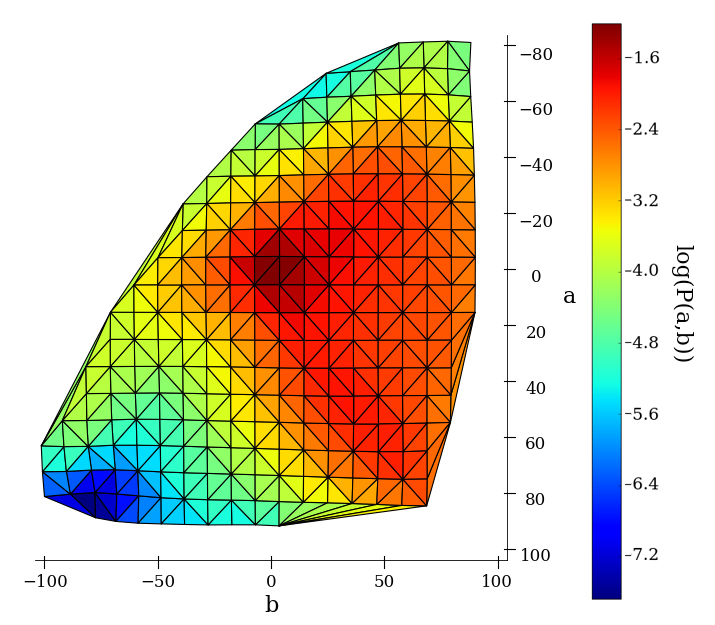
\includegraphics[width=0.48\textwidth]{hist}
	\end{center}
	\caption{\color{red} The histogram of the total fruit dataset}
	\vspace{-10pt}
\end{wrapfigure}





